\documentclass{article}
\usepackage{tikz}
\usetikzlibrary{arrows.meta}

\begin{document}

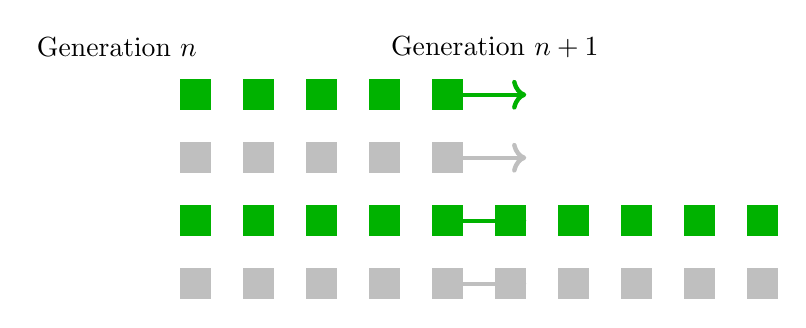
\begin{tikzpicture}[scale=0.8]
    \node at (0,4) {Generation $n$};
    \node at (6,4) {Generation $n+1$};

    % Draw the first row (best genes)
    \foreach \x in {1,...,5} {
        \fill[green!70!black] (\x,3) rectangle ++(0.5,0.5);
    }
    \draw[->, ultra thick, green!70!black] (5.5,3.25) -- (6.5,3.25);

    % Draw the second row (worst genes)
    \foreach \x in {1,...,5} {
        \fill[gray!50] (\x,2) rectangle ++(0.5,0.5);
    }
    \draw[->, ultra thick, gray!50] (5.5,2.25) -- (6.5,2.25);

    % Draw the third row (crossovers)
    \foreach \x in {1,...,5} {
        \fill[green!70!black] (\x,1) rectangle ++(0.5,0.5);
    }
    \foreach \x in {6,...,10} {
        \fill[green!70!black] (\x,1) rectangle ++(0.5,0.5);
    }
    \foreach \x in {1,...,5} {
        \fill[gray!50] (\x,0) rectangle ++(0.5,0.5);
    }
    \foreach \x in {6,...,10} {
        \fill[gray!50] (\x,0) rectangle ++(0.5,0.5);
    }

    % Draw the arrows for crossover
    \draw[->, ultra thick, green!70!black] (5.5,1.25) -- (6.5,1.25);
    \draw[->, ultra thick, gray!50] (5.5,0.25) -- (6.5,0.25);
\end{tikzpicture}

\end{document}